\section{Mininet y Mininet-WiFi}
\label{sec:mininet}

En esta sección se abordará el marco teórico relacionado con las principales herramientas de emulación utilizadas en este proyecto. Se prestará especial atención a Mininet, que es la herramienta principal y la base sobre la cual han surgido otras herramientas de emulación, como Mininet-WiFi y Mininet-IoT.\\

\subsection{Mininet}

Mininet es una herramienta utilizada para emular redes, principalmente del tipo SDN (Software-Defined Networking). Permite emular hosts, routers, switches y enlaces en una sola máquina a un coste reducido, siempre y cuando se cuente con el Kernel de Linux en dicha máquina. Para lograr esto, Mininet utiliza una forma de virtualización "ligera" que aprovecha las capacidades del Kernel de Linux para virtualizar recursos, como las \textit{Namespaces} (consultar \ref{namespaces}) \cite{lantz2010network}.\\
\\
La cantidad de recursos virtualizados dependerá de las características de cada nodo, y esto también afectará el rendimiento de la emulación. Por ejemplo, los nodos tipo \texttt{Host} en Mininet requieren el uso de una \textit{Network Namespace}, lo que les proporciona su propio \textit{stack} de red y los hace completamente independientes\footnote{En lo que respecta a Networking} del sistema y otros nodos en la red emulada. Sin embargo, por defecto, todos los nodos \texttt{Host} comparten el sistema de archivos, la numeración de procesos (PIDs), los usuarios, etc. En términos técnicos, no están completamente aislados como un host real. Esto se debe a que Mininet virtualiza solo los recursos necesarios para llevar a cabo la emulación, lo que mejora el rendimiento y permite que máquinas con recursos limitados puedan realizar la emulación \cite{lantz2010network}.\\
\\
En cuanto a la creación de topologías en Mininet, existen dos enfoques. El primero es utilizar la API escrita en Python para interactuar con las clases de Mininet. Con esta API, se puede construir la topología importando los módulos y clases necesarios para definirla en un script de Python. El segundo enfoque es utilizar la herramienta llamada \textbf{MiniEdit}, que proporciona una interfaz gráfica (GUI) donde los usuarios pueden crear la topología arrastrando y soltando nodos de red. Desde la misma GUI, se puede exportar la topología generada a un archivo (\texttt{*.mn}) para recuperarla más tarde o a un script en Python (\texttt{*.py}) para cargarla en el intérprete de Python cuando sea necesario. Esta herramienta es especialmente útil para aquellos que no tienen conocimientos de programación en Python pero desean utilizar el emulador, lo que representa una ventaja significativa \cite{lantz2010network}.\\

Por lo tanto, se puede concluir que los aspectos más fuertes de Mininet son los siguientes puntos:

\begin{itemize}
    \item Mininet es rápido gracias a su diseño basado en \textit{Namespaces}, lo que permite una gestión eficiente de los recursos. En la sección \ref{namespaces}, se explica cómo se lleva a cabo esta gestión.
    \item Mininet no consume recursos en exceso, ya que virtualiza únicamente los componentes necesarios para la emulación. Además, se pueden establecer límites máximos de recursos para la emulación en caso de ser necesario.
    \item Mininet brinda libertad al usuario para crear topologías y escenarios personalizados utilizando la API en Python de Mininet. Estos escenarios pueden ser fácilmente transferidos a otra máquina, ya que solo se requiere compartir el script que describe la topología. Es importante tener en cuenta que los resultados de las pruebas pueden variar entre diferentes máquinas, ya que Mininet emula la red en lugar de simularla. Por lo tanto, los resultados dependerán de las condiciones de la máquina donde se ejecuten las pruebas.
\end{itemize}

Aunque Mininet ofrece muchas ventajas, también tiene una limitación importante que debe tenerse en cuenta. Como se mencionó anteriormente, Mininet utiliza una forma de virtualización ``ligera" basada en las \textit{Namespaces} del Kernel de Linux. Si bien esta decisión de diseño proporciona beneficios significativos en términos de rendimiento al aprovechar el propio sistema operativo para virtualizar recursos, surge un problema cuando se intenta exportar el emulador a otra plataforma con un sistema operativo diferente. Es posible que este sistema operativo no admita un equivalente funcional a las \textit{Namespaces} de Linux o, incluso si lo hace, su API para utilizarlas puede ser completamente diferente. Esto puede dificultar o incluso impedir la ejecución de Mininet en plataformas que no porten el kernel de Linux.


\subsection{Funcionamiento de Mininet}

Se ha introducido anteriormente que Mininet hace uso de \textit{Network Namespaces} como método para virtualizar \textit{stacks} de red independientes entre sí, y así poder emular redes a un coste mínimo. En la figura \ref{fig:mininet_arch}, se puede ver la arquitectura interna de Mininet para una topología compuesta de dos \texttt{Host}, y de un soft-switch conectado por TCP a un controlador remoto.\\
\par
Como se puede apreciar los host están aislados en sus propias \textit{Namespaces}, y en este caso el switch está corriendo en la \textit{Namespace} por defecto (root). El mecanismo para comunicar a los nodos de esta topología como se adelantaba anteriormente son las \gls{veth}s (Ir a \ref{linuxVeths}), las cuales permitirán emular los enlaces entre los distintos nodos de la red.\\


\begin{figure}[ht]
    \centering
    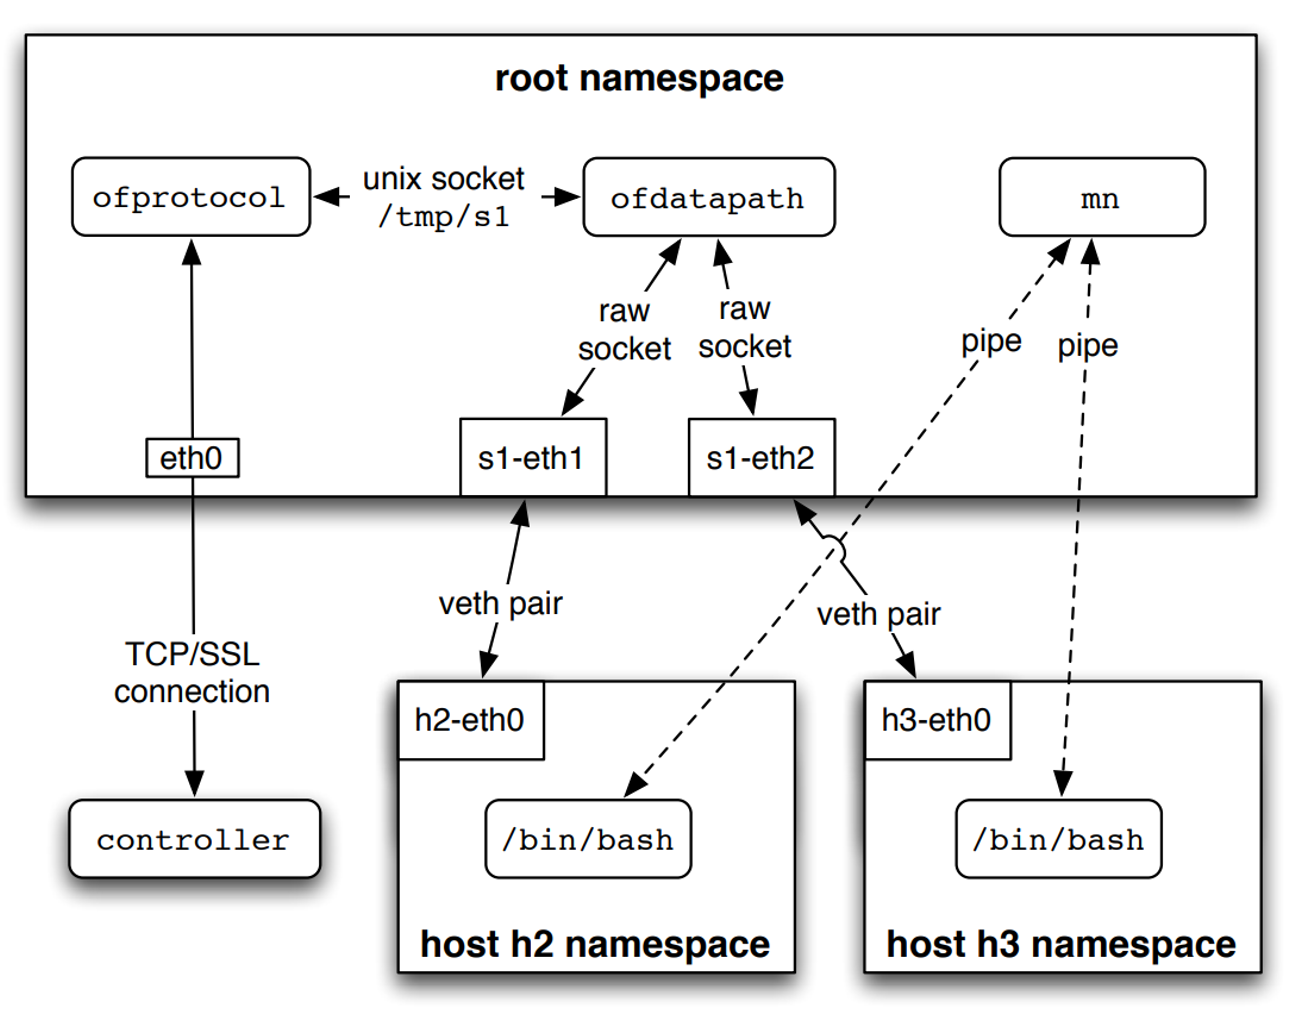
\includegraphics[width=11.5cm]{archivos/img/teoria/mn_arch.png}
    \caption{Arquitectura de Mininet \cite{heller2013reproducible}}
    \label{fig:mininet_arch}
\end{figure}

Una vez expuesta toda la teoría sobre Mininet, podría surgir la siguiente pregunta, ¿Cómo se puede comprobar que realmente hace uso de \textit{Network Namespaces}? Lo primero que se debe hacer es levantar el escenario para que así, Mininet cree las \textit{Network namespaces} que tenga que crear. En este caso, se utilizará la topología expuesta en la figura \ref{fig:mininet_arch}, para levantar dicha topología únicamente se tiene que tener Mininet instalado y seguir los pasos que se indican el bloque \ref{code:scenarioMininet}.


\begin{lstlisting}[language= bash, style=Consola, caption={Levantamiento de la topología de ejemplo},label=code:scenarioMininet]
    # Por defecto siempre carga la topología descrita en la figura anterior
    sudo mn
    
\end{lstlisting}
\vspace{0.5cm}

\begin{figure}[ht]
    \centering
    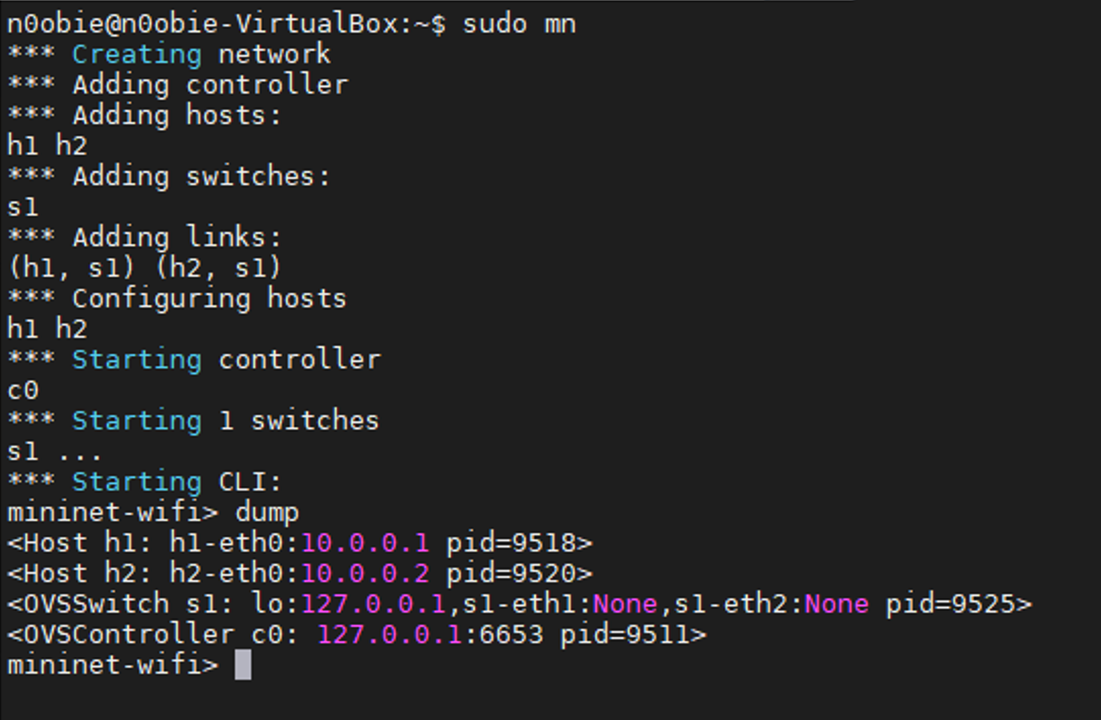
\includegraphics[width=9.5cm]{archivos/img/teoria/mn_01.png}
    \caption{Topología de ejemplo levantada}
    \label{fig:mininet_01}
\end{figure}

Ahora que ya se ha levantado el escenario se debería ser capaces de poder ver si hay \textit{Network Namespaces} en el sistema, para ello se hará uso del \textit{pack} de herramientas iproute2 (Ir a \ref{iproute2}). El comando por excelencia para listar las \textit{Network Namespaces} haciendo uso del módulo \textbf{netns} se puede ver en el bloque \ref{code:MininetNs}.


\begin{lstlisting}[language= bash, style=Consola, caption={Listar Network Namespaces},label=code:MininetNs]
    sudo ip netns list
\end{lstlisting}
\vspace{0.5cm}

\begin{figure}[ht]
    \centering
    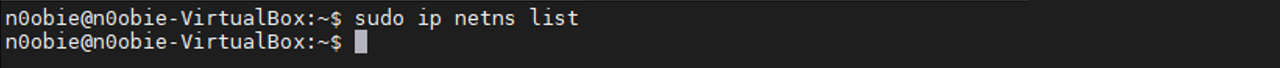
\includegraphics[width=15.5cm]{archivos/img/teoria/mn_02.png}
    \caption{Listado de Network Namespaces existentes en el sistema}
    \label{fig:mininet_02}
\end{figure}

Según se puede apreciar en la figura \ref{fig:mininet_02}, no parece que haya ninguna \textit{Network Namespace} en el sistema, pero entonces, ¿Dónde está el problema? El problema de que el comando \texttt{ip netns list} no arroje información, es que Mininet no está creando el \textit{softlink} requerido para que la herramienta sea capaz de listar las \textit{Network Namespaces}. Atendiendo a la documentación del comando se puede averiguar que dicho comando lee del path \texttt{/var/run/netns/} donde se encuentran todas las \textit{Network Namespaces} con nombre\footnote{Aquellas Netns las cuales se ha hecho un bindmount con su nombre en ese directorio para que persistan aunque no haya ningún proceso corriendo en ellas.}.\\
\par
Como ya se explicó, las \textit{Namespaces} tienen una vida finita, éstas viven siempre y cuando estén referenciadas (Ir a \ref{tab:linux_ns}), por tanto, si ninguna condición de referenciación se cumple, la \textit{Namespace} en cuestión es eliminada.\\
\par
Mininet se encarga de recrear la red emulada, y cuando el usuario termine la emulación, la red emulada debe desaparecer, este proceso debe ser lo más ligero y rápido posible para así ofrecer una mejor experiencia al usuario. La naturaleza del diseño de Mininet incita a pensar que la creación y destrucción de las \textit{Network Namespace} vienen asociadas a la primera condición de refereciación de una \textit{Namespace}. \\
\par
Es decir, no tendría sentido hacer \textit{mounts} ni \textit{softlinks} que a posteriori se deberán eliminar, ya que supondría una carga de trabajo bastante significativa para emulaciones de redes grandes y un aumento del tiempo destinado a la limpieza del sistema una vez que la emulación haya terminado. Además, se debe tener en cuenta que existe una condición que es bastante idónea con las necesidades de Mininet, ya que solo es necesario un proceso corriendo por cada \textit{Network Namespace}, y a la hora de limpiar únicamente se debe terminar con los procesos que sostienen las \textit{Network Namespace}. Cuando ya no haya ningún proceso corriendo en la \textit{Namespace}, y el Kernel se encargará de eliminar las \textit{Namespaces}.\\
\par
Según el razonamiento expuesto, se debería ver varios procesos que son creados a la hora del levantamiento del escenario en Mininet. Estos procesos deberán tener cada uno un fichero de \textit{Network Namespace}, \texttt{/proc/\{pid\}/ns/net}, con un \textit{inode} distinto para aquellos procesos que corren en distintas \textit{Network Namespaces}.\\

\begin{figure}[ht]
    \centering
    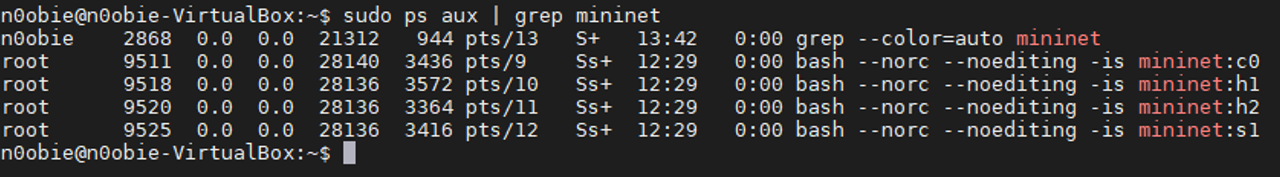
\includegraphics[width=15.5cm]{archivos/img/teoria/mn_03.png}
    \caption{Listado de procesos asociados a Mininet}
    \label{fig:mininet_03}
\end{figure}

Si se inspecciona el fichero \texttt{/proc/\{pid\}/ns/net} para cada proceso indicado en la figura \ref{fig:mininet_03} se podrá ver cuales de ellos están en una \textit{Network Namespace} distinta, en función del valor que tenga el \textit{inode}. Por ejemplo, se va a comprobar los procesos asociados a los \texttt{Host1} y \texttt{Host2}.\\
\par

\begin{figure}[ht]
    \centering
    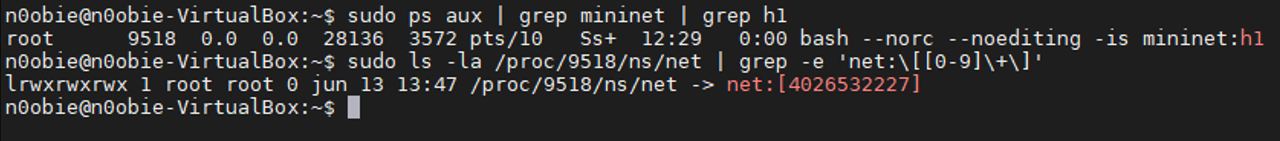
\includegraphics[width=15.5cm]{archivos/img/teoria/mn_04.png}
    \caption{Información relativa al proceso del Host1}
    \label{fig:mininet_04}
\end{figure}

\newpage

\begin{figure}[ht]
    \centering
    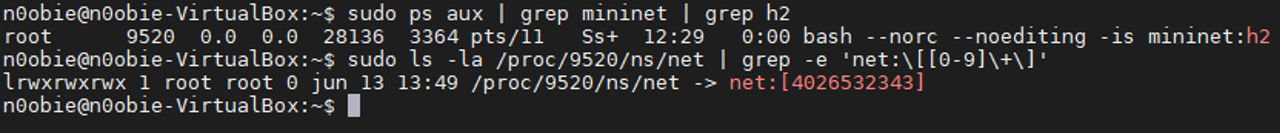
\includegraphics[width=15.5cm]{archivos/img/teoria/mn_05.png}
    \caption{Información relativa al proceso del Host2}
    \label{fig:mininet_05}
\end{figure}

Como se puede ver, \textit{inode} distintos, ficheros distintos, distintas \textit{Network namespaces}. Con esta prueba se puede ver como Mininet hace uso de procesos de bash para sostener las \textit{Network Namespaces} de los nodos que lo requieran.


\subsection{Mininet-WiFi}

Mininet-WiFi \cite{7367387} es un emulador de redes inalámbricas diseñado principalmente para trabajar bajo el estándar \texttt{ieee80211}. Esta herramienta nació de Mininet, es decir, es un \textit{fork} de la misma. Por ello, comparten todas las bases sobre virtualización ``ligera" haciendo uso de \textit{Namespaces} y \gls{veth}s, por tanto, todos los scripts de Mininet son compatibles en Mininet-WiFi. \\
\par
Esto es así ya que toda la funcionalidad wireless es un añadido sobre la base que desarrollaron para Mininet. Los desarrolladores de Mininet-WiFi se valieron del subsistema wireless del Kernel de Linux y del módulo mac80211\_hwsim, para conseguir emular las interfaces y el supuesto medio inalámbrico. Para más información sobre esta herramienta se recomienda ir al \textbf{punto} \ref{mn-wifi_bmv2_integration}, donde se hace un análisis profundo sobre las jerarquías de clases añadidas en Mininet-WiFi, como opera internamente y como se comunica con el módulo en el kernel para generar los escenarios inalámbricos.



\subsection{Mininet-IoT}
\label{mininetIoT}

La herramienta Mininet-IoT \cite{mininetIOT} es un emulador de redes de baja capacidad diseñado para trabajar en conjunto bajo el estándar \texttt{ieee802154} y la capa de adaptación 6LoWPAN. Esta herramienta nació de Mininet-WiFi, que a su vez nació de Mininet, por lo que en la práctica, Mininet-IoT comparte todas las técnicas de virtualización ``ligera" de Mininet. Al heredar de Mininet-WiFi y Mininet, todos los scripts para desplegar topologías alámbricas y WiFi son compatibles en Mininet-IoT.  \\
\par

La gran diferencia entre Mininet-IoT y Mininet-WiFi, radica en el módulo que emplean para conseguir emular las interfaces y el supuesto medio inalámbrico. Mininet-WiFi hace uso del módulo mac80211\_hwsim, mientras que Mininet-IoT hace uso del módulo del Kernel mac802154\_hwsim (es necesario tener una versión del Kernel superior a la \texttt{4.18.x} para obtener dicho modulo). Toda la gestión de nodos, interfaces y enlaces es exactamente la misma a la de Mininet-WiFi. Por ello, Ramon Fontes (principal desarrollador de la herramienta), creó una clase agnóstica para gestionar módulos del Kernel en Mininet-WiFi, y migró todo el proyecto de Mininet-IoT a Mininet-WiFi. De esta forma, el mantenimiento del \textit{core} que compartían ambas herramientas se hacía únicamente en un proyecto, y daba la posibilidad al usuario de Mininet-WiFi de establecer enlaces de baja capacidad en sus topologías inalámbricas.